\chapter{Turbulently-Driven Detonation Mechanism}

\section{Carbon Detonation}

In our previous work, we determined that our turbulently-driven detonation mechanism can lead to the detonation of carbon in electron-degenerate matter. Three-dimensional hydrodynamic simulations were carried out with electron-degenerate fuel consisting of equal ratios of carbon and oxygen in a density of $10^7$ g cm$^{-3}$. Through extensive statistical tests, detonation initiation occured when the time scale of the turbulence, characterized by the eddy-turnover time on the critical length scale, becomes larger than the nuclear burning timescale, $t_{edd}/t_{burn} \simeq 10^9$.

\begin{table}[htp]
\caption[A table of carbon-oxygen runs with different resolution, RMS velocity and mean temperature..]{Results from intitial work that established a turbulently-driven detonation mechanism using only carbon and oxygen. Mass-weighted mean temperature at the time of detonation in each resolution are listed.}
  \begin{center}
      \begin{tabular}{|c|c|c|c|}
        \hline
	      Resolution & $T_{mean}$(K) \\
        \hline\hline
        $64^3$   & $1.12 \times 10^9$ \\
	$128^3$   & $1.17 \times 10^9$ \\
	$256^3$   & $1.17 \times 10^9$ \\
	$512^3$   & $1.18 \times 10^9$ \\      
        \hline
   \end{tabular}
  \end{center}
  \label{runs}
\end{table}

\begin{center}
\begin{figure}[hp]

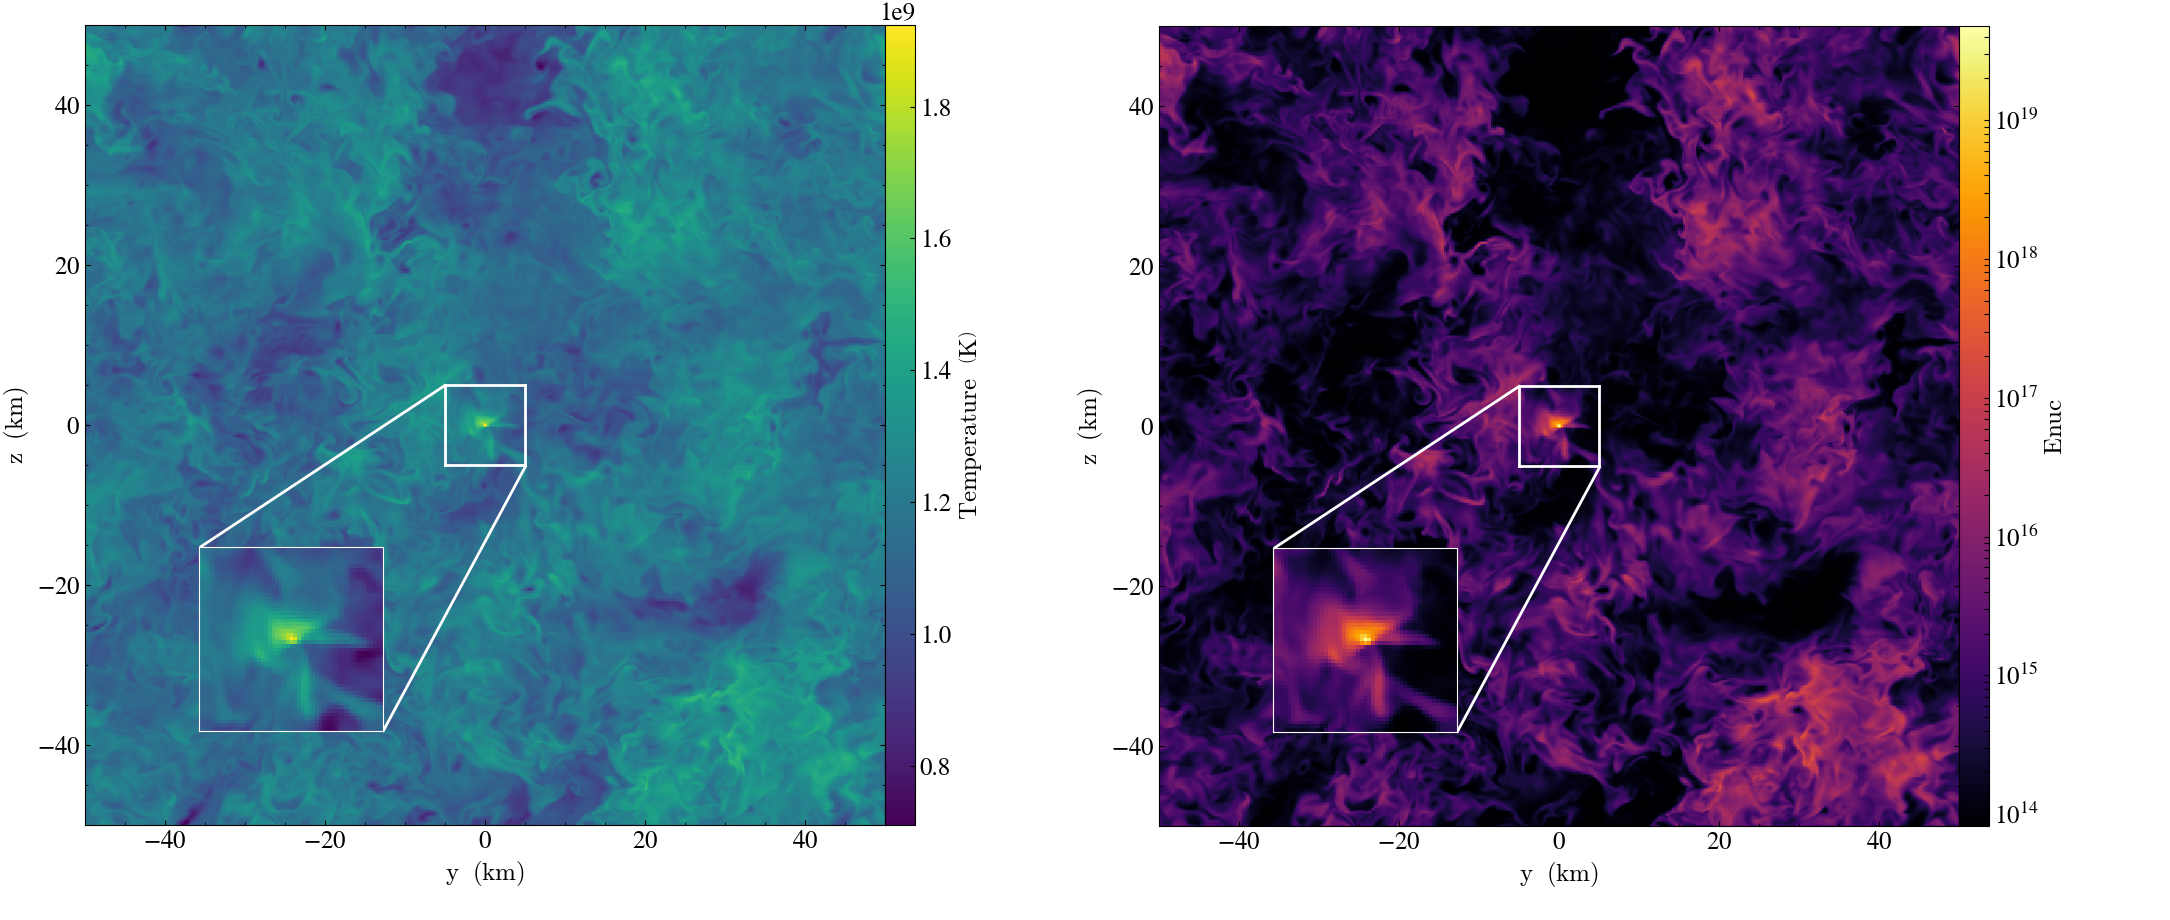
\includegraphics[width=1.0\textwidth]{combined_slice_carbon.png}
\centering
\caption[Slice plots of temperature and specific nuclear energy generation rate, through the maximum temperature in the $z$-$y$ plane, for the $512^3$ run]{Slice plots of temperature and specific nuclear energy generation rate from the C/O run, through the x-axis in the $z$-$y$ plane, for the $512^3$. Each is centered about the hot spot just before leading into a detonation.}
\label {fig:temp_enuc}

\end{figure}
\end{center}

An important implication of these runs is that detonation of carbon can occur in the distributed burning regime through our turbulence mechanism. This is especially important since the Zel'dovich gradient mechanism has been the leading mechanism explaining spontaneous detonation initiation in SNe Ia. Although not wrong, it lacks the physics of turbulence which we know must play a role in the DD channel. From these results, we can now utilize our new mechanism to explore other parameters within these mergers.

\section{Helium Detonation}

Having now a successful detonation mechanism, incorporating helium is a natural next step. As explained before, the detonation of the helium layer of the primary WD opens up the parameter space of how the carbon core can be detonated. Previous work done by Holcomb and collaborators determined tight constraints with regards to temperature, density, and critical length scales for helium burning based upon the Zel'dovich gradient mechanism \cite{holcomb}. They performed one-dimensional hydrodynamic simulations with various initial conditions similar to that which can be modeled with SNe Ia progenitor models. With a turbulently-driven detonation mechanism, we now can perform three-dimensional hydrodynamic simulations and explore the constraints previously modeled.

\section{Simulation Methodology}

Computational tools were used to analyze the physics of turbulence. FLASH, a multiphysics multiscale code built for high-energy density physics, was used to execute three-dimensional hydrodynamic simulations. The hydrodynamics solver used in this case was the split piece-wise parabolic method (PPM). The Helmholtz equation of state was used to incorporate the contributions from nuclei, electrons, blackbody photons, electron-degeneracy, and relativistic effects \cite{timmeswoosley92}. Since this work is only considering a small number of nuclear species, a 19-isotope network was used \cite{weaveretal78}, \cite{timmes99}.

In all, 18 simulations were conducted. Each one had a domain size of $L$ = 100 km, simulated in a fully-periodic box. Spatial resolution ranged from $128^3$ ($L$), $256^3$ ($M$), and $512^3$ ($H$) cells, on a uniform grid. Within each resolution, the parameter space of density and nuclear composition was explored. Densities were set to $10^5$ (LowDen) and $10^6$ (HighDen) g cm$^{-3}$. Initial helium abundance varied from 100\% (PureHe), 25\% (MedHe), and 10\% (MinHe). Carbon and oxygen took up the remaining portion with an assumed equal ratio to one another for each simulation. Initial temperature in all simulations began at $10^8$ K. 

Simulations begin with all the fluid having zero velocity. A large-scale stochastic forcing routine is then used as a stirring mechanism to increase the momentum of the simulation. Each simulation runs until the RMS velocities reach a stable value, indicating that it has reached steady-state turbulence. At this point, the simulations are restarted with nuclear burning turned on and are continued to determine whether detonation will occur. Detonation was classified as the time where helium abundance dropped by 10\% of initial value.

\section{Simulation Results}

Slice plots were generated for temperature and specific nuclear burning using the highest resolution models, $512^3$. A snap shot is taken at the time when the detonation has initiated, with the box centered about the point of maximum temperature, which, owing to the extreme sensitivity of the rates to temperature, is also the point of maximum nuclear burning. At this angle, one is looking through the $x$-axis on the $z$-$y$ plane. Each slice plot has an inset which is zoomed in on the hotspot.

Figure 2.2 shows the slice plots for the MinHeLowDen\_H run, which has a $v_{\rm rms} = 1.26 \times 10^8$ cm s$^{-1}$. For all resolutions, these runs fully detonated helium but saw an increase in carbon abundance, while keeping oxygen almost steady. This implies that the helium was burnt off through the triple-alpha process into carbon. Carbon abundances showed no signs of coming to a detonation.

Figure 2.3 shows the slice plots for the MedHeLowDen\_H run, which has a $v_{\rm rms} = 1.28 \times 10^8$ cm s$^{-1}$. Similar to the previous set of parameters, these runs also saw complete detonation of helium with an increase in carbon, while keeping oxygen steady. This also implies that the triple-alpha process fused most of the helium into carbon, while showing no signs of a carbon detonation.

Figure 2.4 shows the slice plots for the PureHeLowDen\_H run. None of these runs, at all resolutions, detonated. However, helium is seen to also burn into carbon through the triple-alpha process. The slice plots are of the last time step recorded, which has a $v_{\rm rms} = 1.25 \times 10^8$ cm s$^{-1}$. A detonation may be observed if simulations ran long enough but this will explored in more detail in future work.

Figure 2.5 shows the slice plots for the MinHeHighDen\_H run, which has a $v_{\rm rms} = 1.22 \times 10^8$ cm s$^{-1}$. All resolutions of these runs saw a detonation of helium and then of carbon shortly afterwards. They also see a rise in oxygen, which implies that on top of the traditional triple-alpha process occuring, an additional alpha capture on carbon occurs to fuse into oxygen.

Figure 2.6 shows the slice plots for the MedHeHighDen\_H run, which has a $v_{\rm rms} = 5.82 \times 10^7$ cm s$^{-1}$. These runs also show complete detonation of helium and carbon with some formation of oxygen, with indications that heavier elements must have been formed post-detonation.

Figure 2.7 shows the slice plots for the PureHeHighDen\_H run, which has a $v_{\rm rms} = 1.25 \times 10^8$ cm s$^{-1}$. These runs see an almost full detonation of helium, with the abundance ratio falling sharply from 100\% to 20\%. At the onset of detonation, carbon abundance rises from \%0 to near 17.5\%, then immediately fully detonates. Oxygen remains steadily at \%0, indicating again that heavier elements have been formed.

\section{Conclusion}

This body of work confirms that turbulently-driven detonation can occur with various abundance levels of helium, carbon, and oxygen. More specifically, the critical temperature for carbon detonation is robustly a factor of $\sim 2-3$ times lower than theorized from previous studies based upon Zel'dovich. Opening up the parameter space of initial conditions for possible detonation scenarios has been an ongoing endeavour for many decades. With newer observational datasets such as \textit{Gaia}, we can now put constraints on our models and also put our focus on specific channels that match these observations. Further work includes exploring more abundance ratios, higher resolutions, and incorporating more in-depth species networks that would allow us to better understand the nucleosynthesis in these simulations.

\begin{center}
\begin{figure}[!htb]

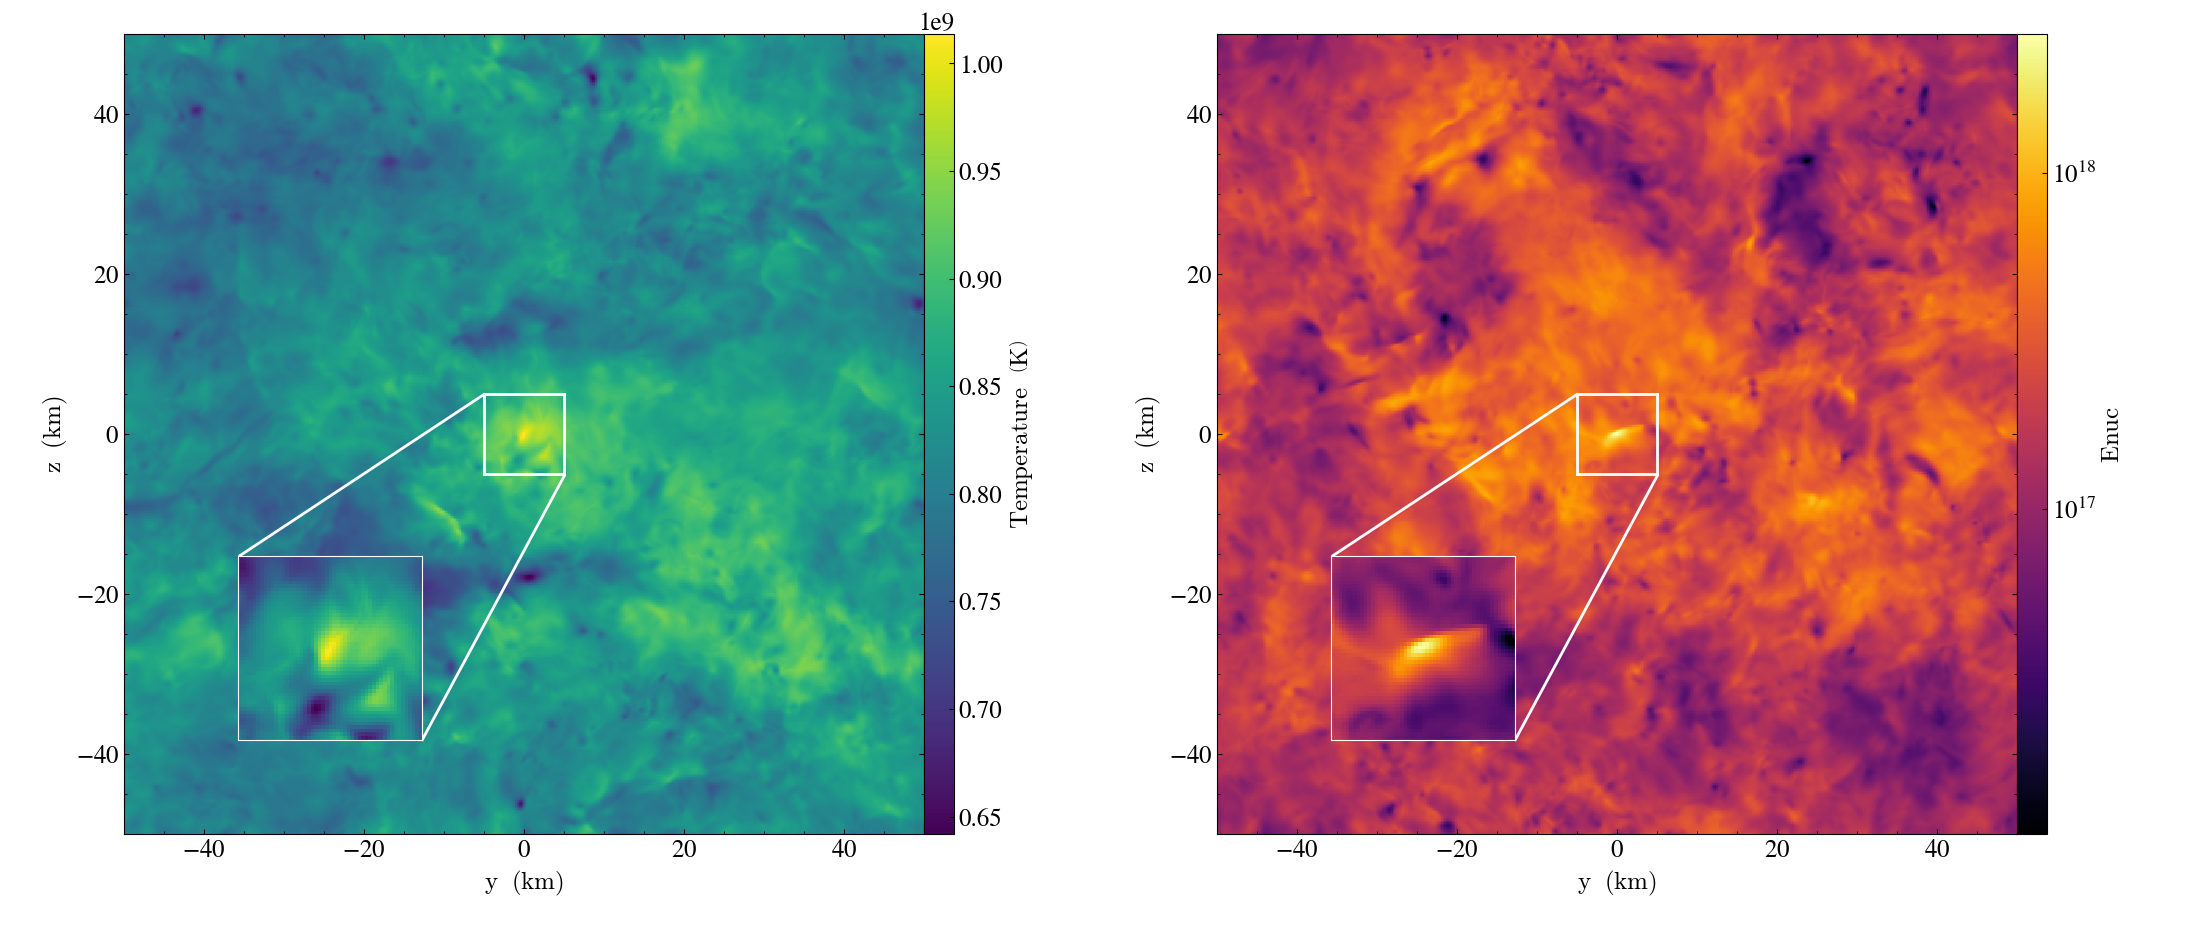
\includegraphics[width=1.0\textwidth]{combined_512_10e5_0.1_new.png}
\centering
\caption[Slice plots of temperature and specific nuclear energy generation rate, for the MinHeLowDen\_H run]{Slice plots of temperature and specific nuclear energy generation rate, for the MinHeLowDen\_H run, through the x-axis in the $z$-$y$ plane, at the onset of detonation.}
\label {fig:temp_enuc}
         
\end{figure}
\end{center}

\begin{center}
\begin{figure}[!htb]

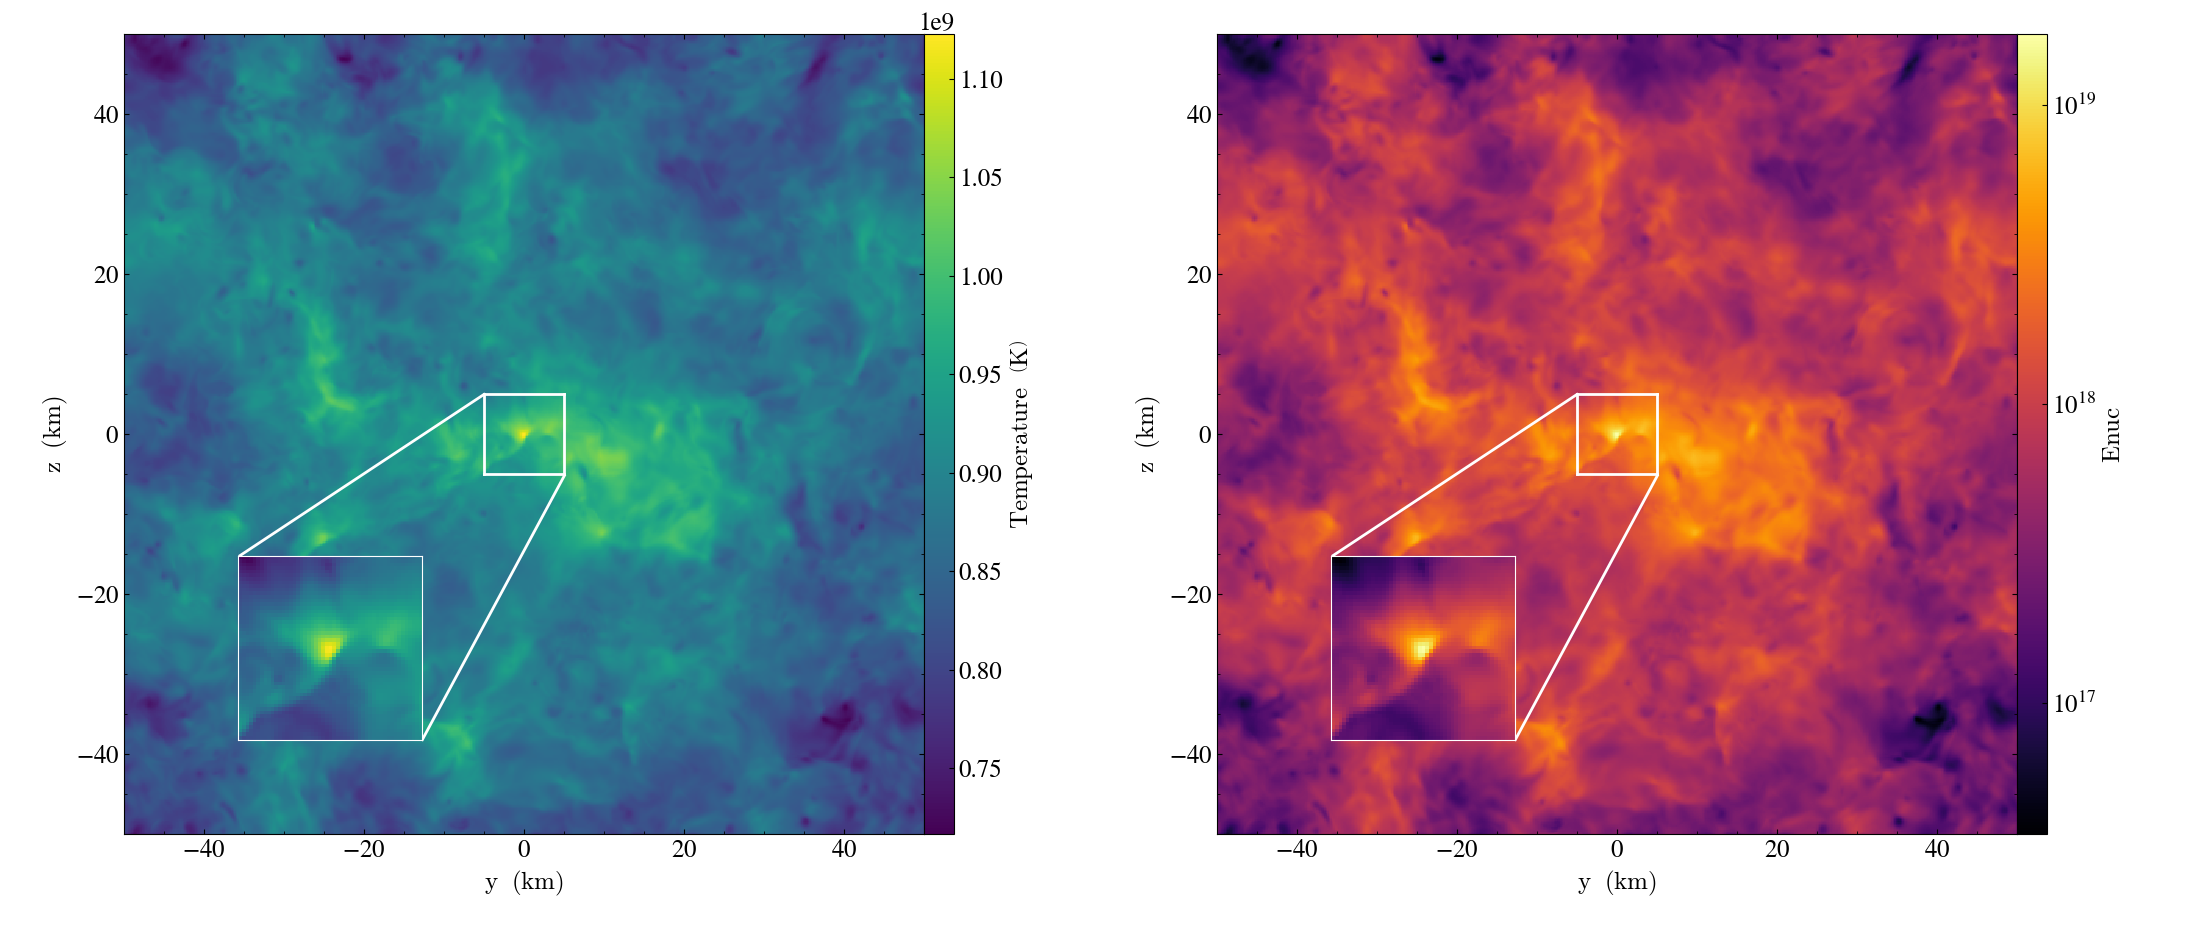
\includegraphics[width=1.0\textwidth]{combined_512_10e5_0.25_new.png}
\centering
\caption[Slice plots of temperature and specific nuclear energy generation rate, for the MedHeLowDen\_H run]{Slice plots of temperature and specific nuclear energy generation rate, for the MedHeLowDen\_H run, through the x-axis in the $z$-$y$ plane, at the onset of detonation.}
\label {fig:temp_enuc}

\end{figure}
\end{center}

\begin{center}
\begin{figure}[!htb]

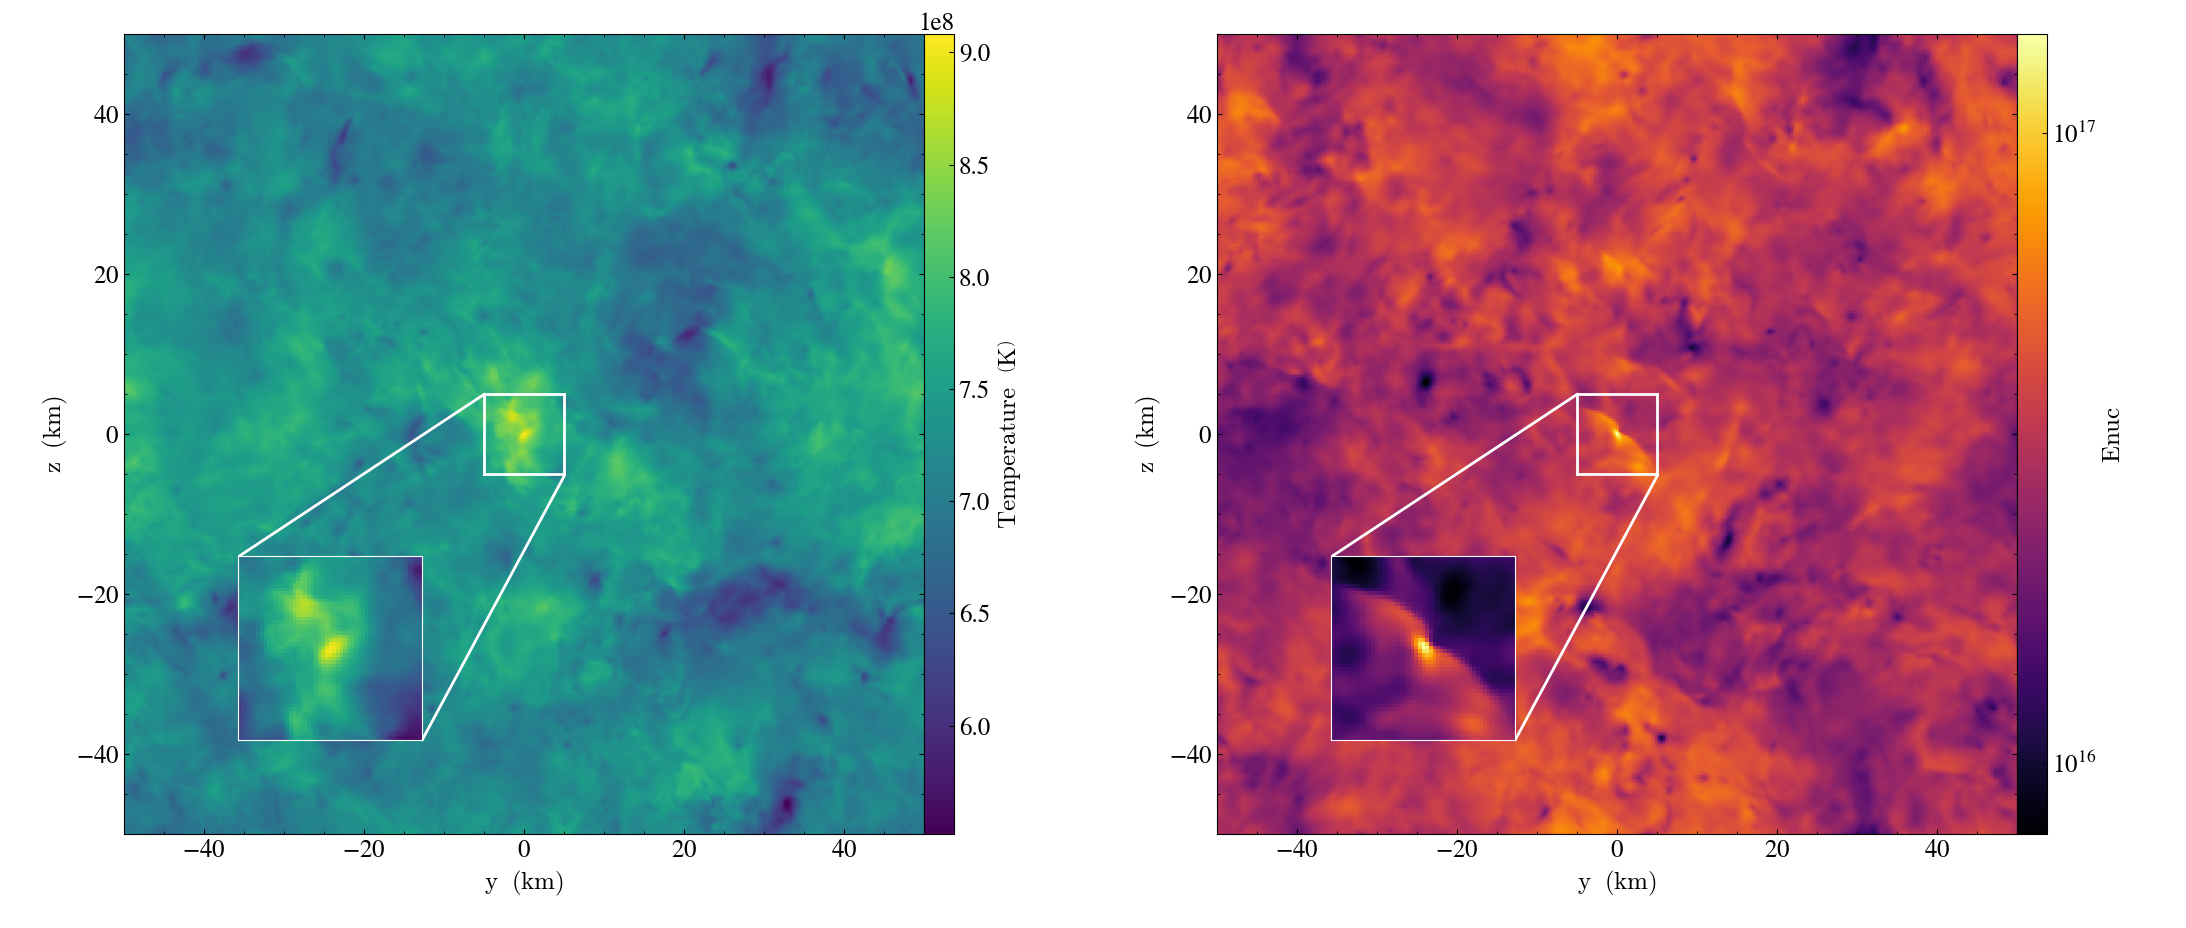
\includegraphics[width=1.0\textwidth]{combined_512_10e5_1.0_new.png}
\centering
\caption[Slice plots of temperature and specific nuclear energy generation rate, for the PureHeLowDen\_H run]{Slice plots of temperature and specific nuclear energy generation ratefor the PureHeLowDen\_H run, through the x-axis in the $z$-$y$ plane, at the last time step of the run.}
\label {fig:temp_enuc}

\end{figure}
\end{center}
\begin{center}
\begin{figure}[!htb]

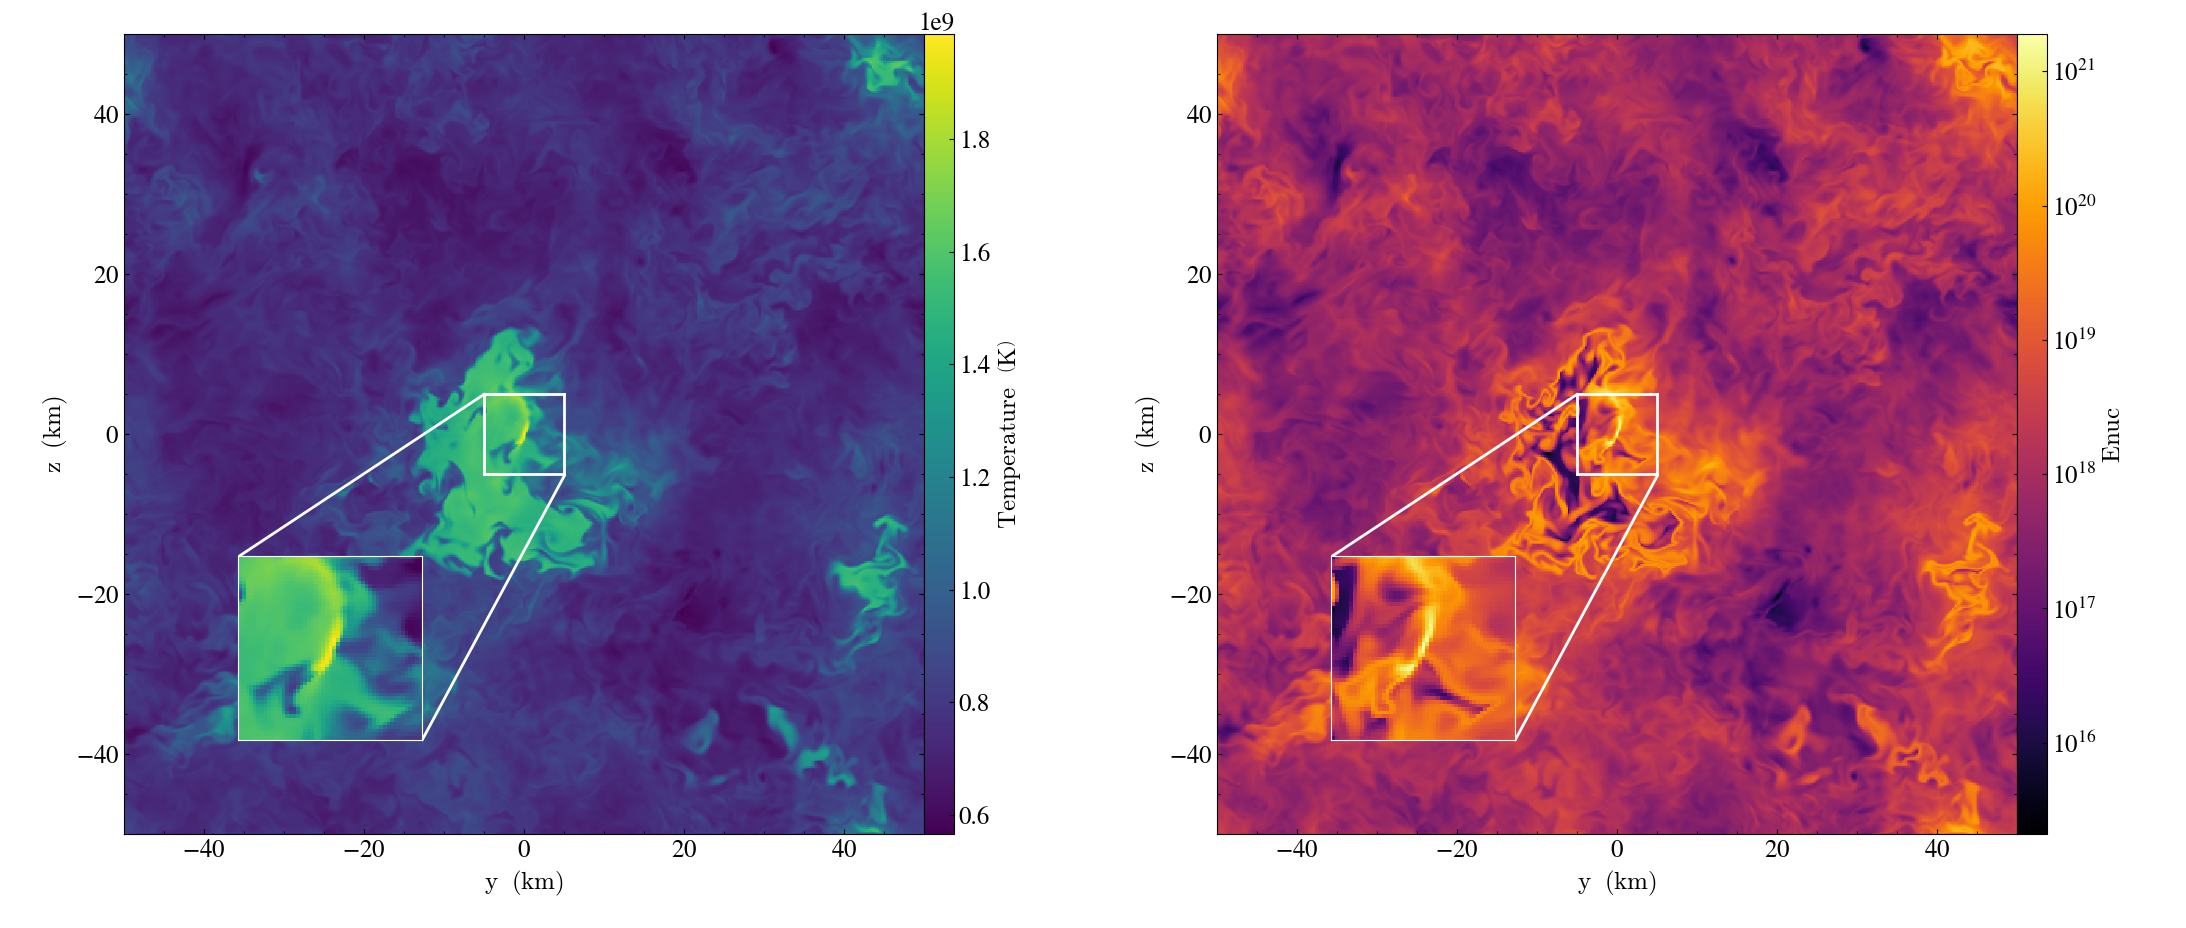
\includegraphics[width=1.0\textwidth]{combined_512_10e6_0.1_new.png}
\centering
\caption[Slice plots of temperature and specific nuclear energy generation rate, for the MinHeHighDen\_H run]{Slice plots of temperature and specific nuclear energy generation rate, for the MinHeHighDen\_H run, through the x-axis in the $z$-$y$ plane, at the onset of detonation.}
\label {fig:temp_enuc}

\end{figure}
\end{center}
\begin{center}
\begin{figure}[!htb]

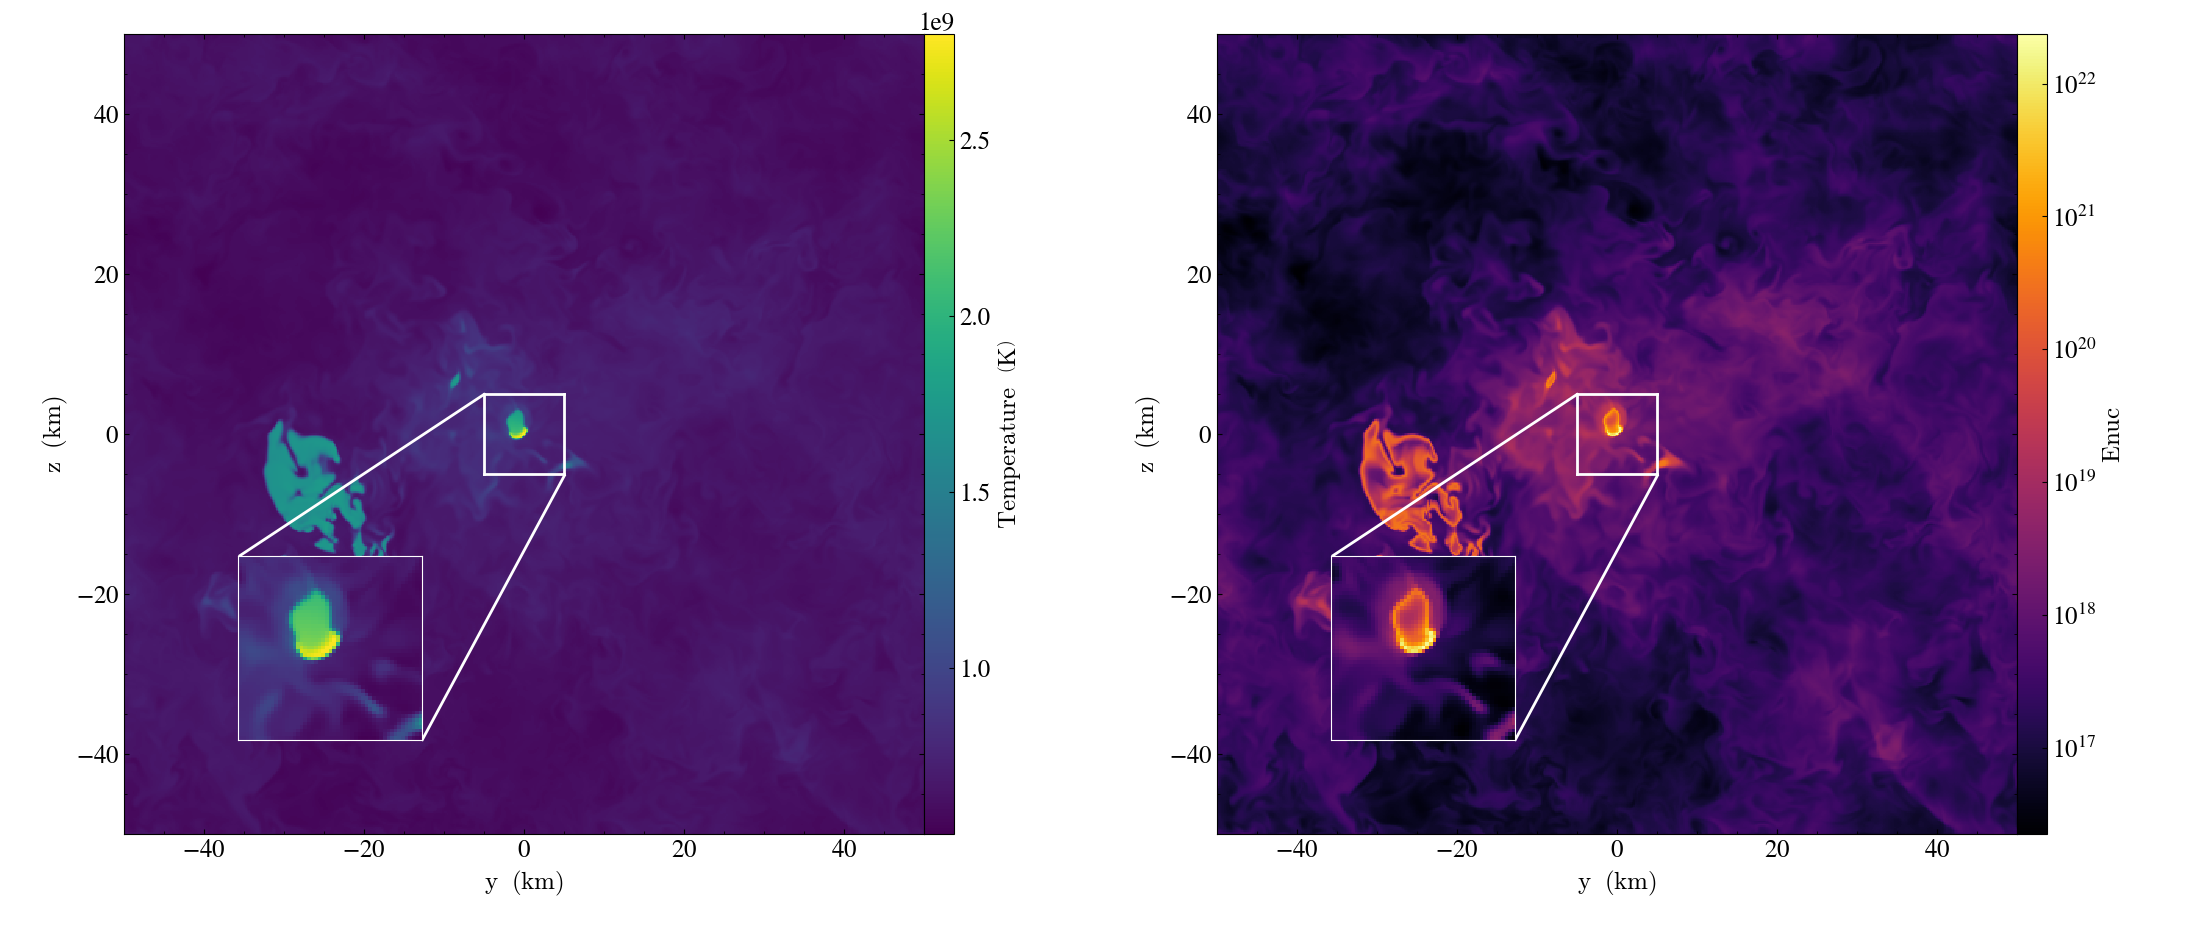
\includegraphics[width=1.0\textwidth]{combined_512_10e6_0.25_new.png}
\centering
\caption[Slice plots of temperature and specific nuclear energy generation rate, for the MedHeHighDen\_H run]{Slice plots of temperature and specific nuclear energy generation rate, for the MedHeHighDen\_H run, through the x-axis in the $z$-$y$ plane, at the onset of detonation.}
\label {fig:temp_enuc}

\end{figure}
\end{center}

\begin{center}
\begin{figure}[!htb]

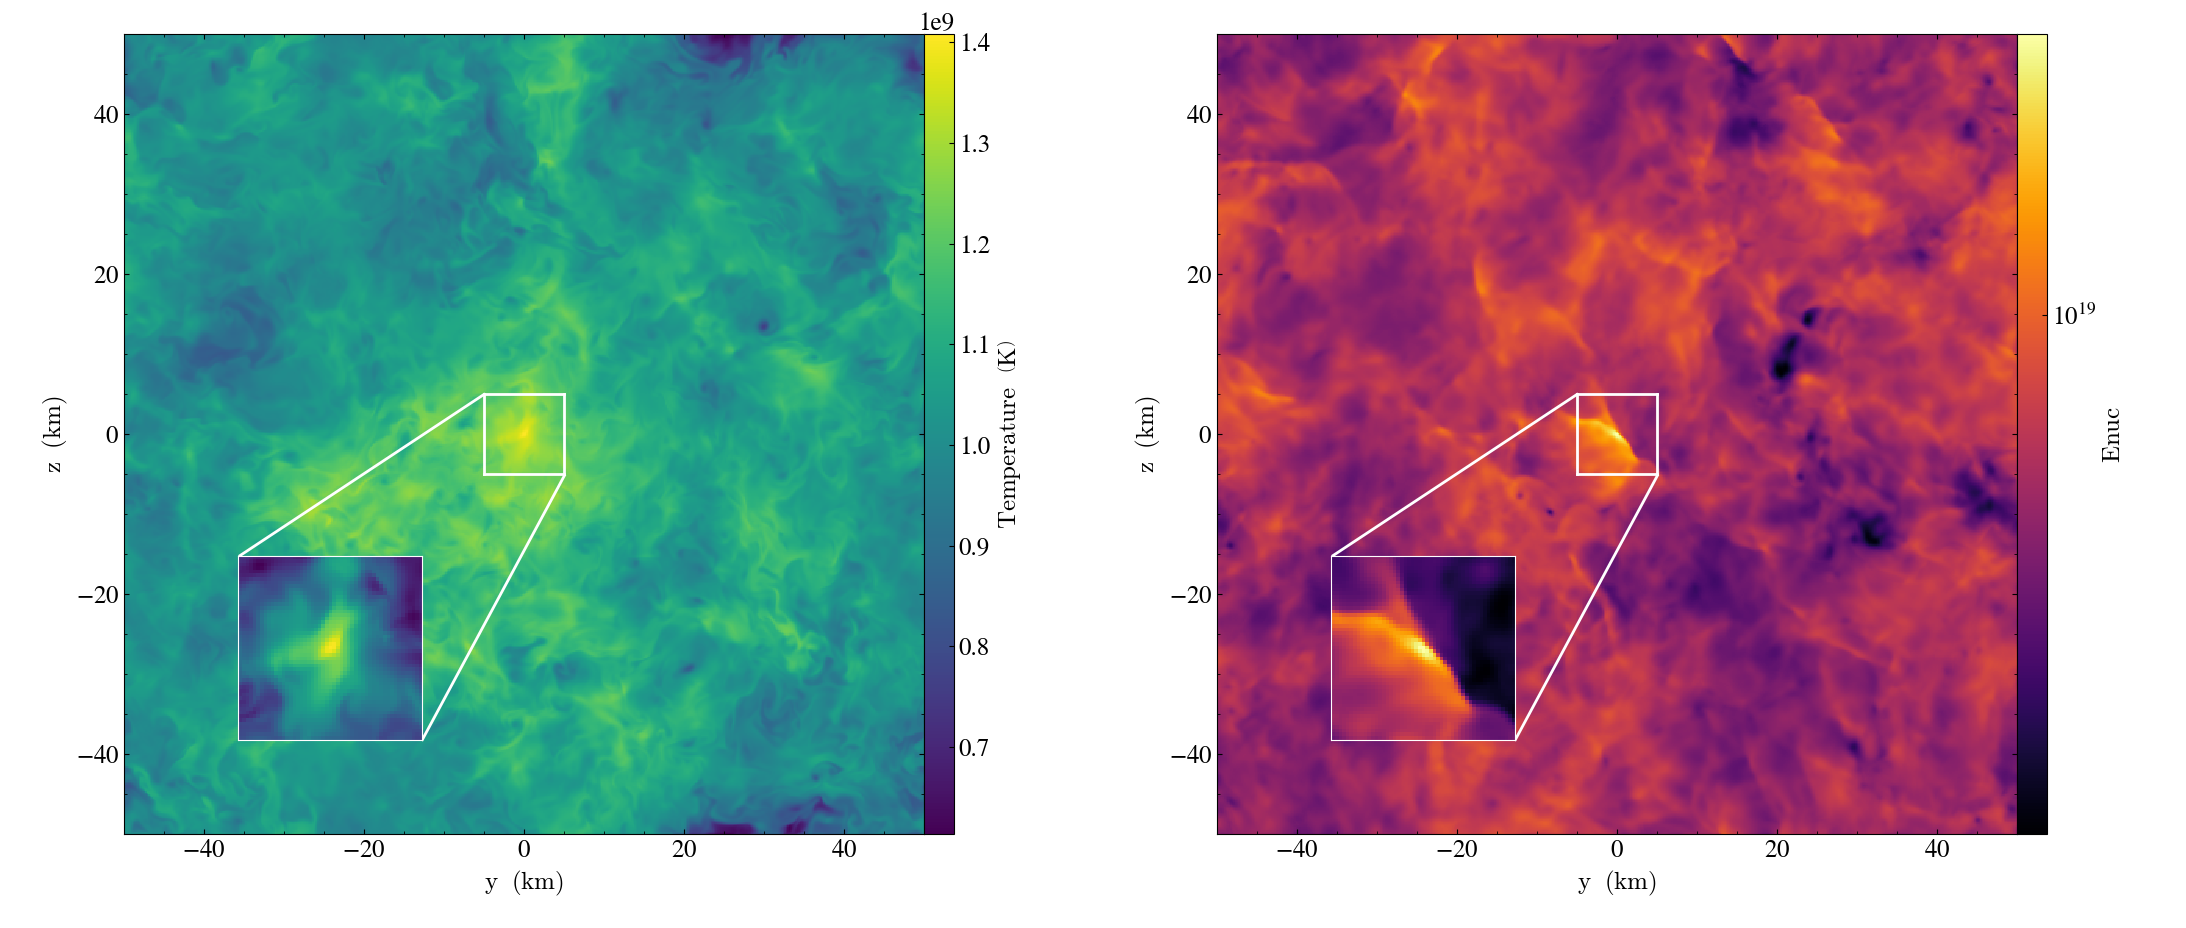
\includegraphics[width=1.0\textwidth]{combined_512_10e6_1.0_new.png}
\centering
\caption[Slice plots of temperature and specific nuclear energy generation rate, for the PureHeHighDen\_H run]{Slice plots of temperature and specific nuclear energy generation rate, for the PureHeHighDen\_H run, through the x-axis in the $z$-$y$ plane, at the onset of detonation.}
\label {fig:temp_enuc}

\end{figure}
\end{center}

\begin{table}[!htb]
        \caption[A table of helium-carbon-oxygen runs with different resolution, RMS velocity and mean temperature..]{A table of runs with the different resolutions, densities, helium abundances, and mean temperature at the time of detonation initiation, $T_{\rm det}$ (K).}
  \begin{center}
      \begin{tabular}{|c|c|c|c|}
        \hline
              Resolution & Density (g cm$^{-3}$) & Helium Abundance & $T_{\rm det}$ (K)\\
        \hline\hline
        $128^3$   & $10^5$ & 0.1 & $8.22 \times 10^8$  \\
        $128^3$   & $10^5$ & 0.25 & $8.77 \times 10^8$  \\
        $128^3$   & $10^5$ & 1.0 & None  \\
        $128^3$   & $10^6$ & 0.1 & $7.80 \times 10^8$  \\
        $128^3$   & $10^6$ & 0.25 & $7.87 \times 10^8$  \\
        $128^3$   & $10^6$ & 1.0 & $9.91 \times 10^8$  \\
        $256^3$   & $10^5$ & 0.1 & $8.25 \times 10^8$  \\
        $256^3$   & $10^5$ & 0.25 & $8.83 \times 10^8$  \\
        $256^3$   & $10^5$ & 1.0 & None  \\
        $256^3$   & $10^6$ & 0.1 & $7.99 \times 10^8$  \\
        $256^3$   & $10^6$ & 0.25 & $8.81 \times 10^8$  \\
        $256^3$   & $10^6$ & 1.0 & $1.09 \times 10^9$  \\
        $512^3$   & $10^5$ & 0.1 & $8.28 \times 10^8$  \\
        $512^3$   & $10^5$ & 0.25 & $8.75 \times 10^8$  \\
        $512^3$   & $10^5$ & 1.0 & None  \\
        $512^3$   & $10^6$ & 0.1 & $7.80 \times 10^8$  \\
        $512^3$   & $10^6$ & 0.25 & $6.30 \times 10^8$  \\
        $512^3$   & $10^6$ & 1.0 & $1.06 \times 10^9$  \\
        \hline
   \end{tabular}
  \end{center}
  \label{runs}
\end{table}

